\documentclass[12pt]{article}

\usepackage{geometry} % Required to change the page size to A4
\geometry{a4paper} % Set the page size to be A4 as opposed to the default US Letter

\usepackage{graphicx} % Required for including pictures

\usepackage{float} % Allows putting an [H] in \begin{figure} to specify the exact location of the figure
\usepackage{wrapfig} % Allows in-line images such as the example fish picture
\usepackage{caption}

\usepackage{lipsum} % Used for inserting dummy 'Lorem ipsum' text into the template

\linespread{1.2} % Line spacing

%\setlength\parindent{0pt} % Uncomment to remove all indentation from paragraphs

\graphicspath{{./Pictures/}} % Specifies the directory where pictures are stored

\begin{document}

%---------------------------------------------------------------------------------
%	TITLE PAGE
%---------------------------------------------------------------------------------

\begin{titlepage}

\newcommand{\HRule}{\rule{\linewidth}{0.5mm}} % Defines a new command for the horizontal lines, change thickness here

\center % Center everything on the page

\HRule \\[0.4cm]
{\large \bfseries A Robust Solution for Echo Server Model}\\[0.4cm] % Title of your document
\HRule \\[1.5cm]

\begin{minipage}{0.6\textwidth}
\begin{flushright}
  \large
Adrian (atrejo),
Dalong Cheng(dalongc) 
\end{flushright}
\end{minipage}
~
\begin{minipage}{0.4\textwidth}
\begin{flushright} \large

\end{flushright}
\end{minipage}\\[4cm]

{\large \today}\\[3cm] % Date, change the \today to a set date if you want to be precise

%\includegraphics{Logo}\\[1cm] % Include a department/university logo - this will require the graphicx package

\vfill % Fill the rest of the page with whitespace



%----------------------------------------------------------------------------------------
%	TABLE OF CONTENTS
%----------------------------------------------------------------------------------------
\end{titlepage}

\tableofcontents % Include a table of contents
\setcounter{page}{2}
\pagenumbering{roman}

\newpage % Begins the essay on a new page instead of on the same page as the table of contents 

%--------------------------------------------------------------------------------
%	INTRODUCTION
%--------------------------------------------------------------------------------

\pagestyle{headings}
\setcounter{page}{1}
\pagenumbering{arabic}

\section{Overview}
In 15440 project 3, we are going to implement a robust solution for
echo server model. The echo client will send to echo manager some echo messages
, upon receiving the echo message, the echo manager will log the message and 
dispatch request to a backend echo server, the echo server will store the echo message, then send identical message back to client. The feautres will be described in following sections in more detail. 

The reason why we choose to implement a echo server is that
we want to focus on design and implement a reliable and solid solution
for distributed system rather than spending too much on application log. 
Since most of the distributed
application can be abstracted as echo server like model, which involving
sending, receiving message and/or sharing state among multiple nodes, we 
can easily extend this project into reliable application, such as 
ticket reservation system, online game, etc.

\begin{figure}[H] % Example image
\center{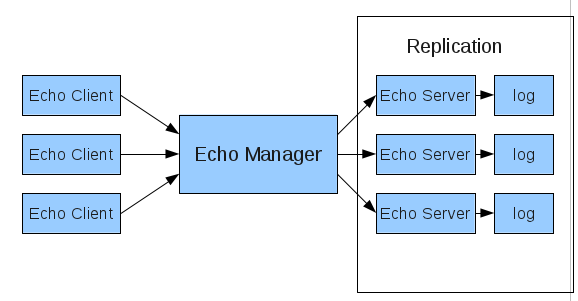
\includegraphics[width=0.5\linewidth]{1.png}}
\caption{General Architecture}
\label{fig:speciation}
\end{figure}

\section{Features}
\subsection{Crash Recovery}
We will use Write-Ahead Logging (WAL) method to enable echo manager recover form
failure. The echo manager will record all the ecoh request it receivevd from echo 
client. The log will contain some meta data for later recovery. When echo manager 
crashes, firtsly, we will analysis the log, then recover the system from the crash. 
\subsection{Job Partition}
The echo manager will dispatch work for all the echo servers. We will use hash ring
method to allocate work to each echo server. The system will also support dynamic
joinning and leaving.
\subsection{Data Replication}
Need discussion

\section{General Design}
The whole system will be developed with Go programming language on Linux 
environment. We divide our work into 3 tiers, each tier will be based on previously work. The first tier will implement the most basic function and the third tier will contain more ``advanced'' function.

\subsection{First Tier}
The first tier will have one echo client, echo manager and echo server. The
echo manager will support crash recovery by using WAL method.  
\begin{figure}[H]
\center{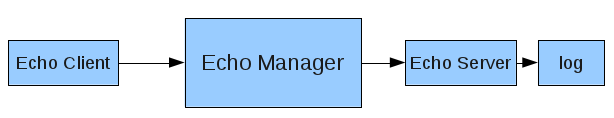
\includegraphics[width=0.5\linewidth]{2.png}}
\caption{First Tier}
\label{fig:speciation}
\end{figure}

\subsection{Second Tier}
The second tier will support multiple echo clients and multiple echo servers. 
We will add feature to enable echo manager to uniformly dispatch the work 
to all the echo server. The echo manager will also need to response appropriately 
to echo server leave and join.
\begin{figure}[H]
\center{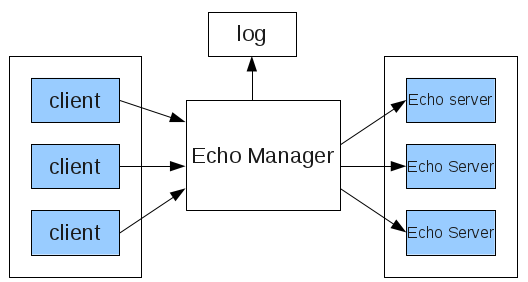
\includegraphics[width=0.5\linewidth]{3.png}}
\caption{Second Tier}
\label{fig:speciation}
\end{figure}

\subsection{Third Tier}
Based on the previous tiers of work, the third tier will further support 
replication among all the echo server. 

\subsection{Component API}
Need discussion here

Echo Client
\begin{itemize}
  \item \texttt{send - send echo message}  
  \item \texttt{reveive - receive echo reply}  
\end{itemize}
Echo Manager
\begin{itemize}
  \item \texttt{join - set track for the player to play}  
\end{itemize}
Echo Server
\begin{itemize}
  \item \texttt{position - indicate conductor to set to given position}
\end{itemize}

\section{Test Plan}
In this project, we have 3 relatively independent component, echo client, 
echo manager and echo server. We will mainly test echo manager and echo
server.

\subsection{Functional Test}
The functional test will test each component independently. We will try to   
cover each function in every component, to garantee it generate expected  
result, given expceted input.

\subsection{Integration Test}
The integration test is to test all the components as whole. Fail recovery,
dynamic node join or leave and replication will be the key test point.

\subsection{Stress Test}
In the stress test, we will create as many echo client as possible to test
the limit of the whole system.

\section{Timeline}
\begin{figure}[H]
\center{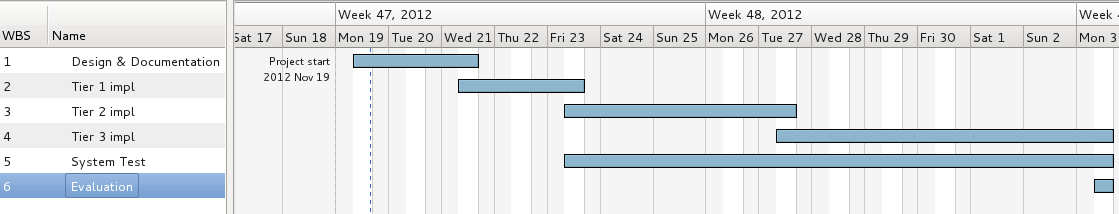
\includegraphics[width=1.1\linewidth]{5.png}}
\caption{Initial Timeline for Project 3}
\label{fig:speciation}
\end{figure}

\section{Evalutation}
Our system should support many echo clients working simultenously and   
making progress. There are several point to evaluate.
\begin{enumerate}
  \item Echo manager will record all the request from client, it 
    should be able to reover from crashing, upon recovery
    it will remain in a consistent system state. 
  \item Echo manager will dispatch the request to different echo server. The 
    load should be balanced among all existed echo servers.
  \item Echo server should support replication feature. 
  \item Echo server can dynamicly join and leave.
\end{enumerate}

\end{document}

